
\documentclass[11pt,a4paper]{article}
\usepackage[T1]{fontenc}
\usepackage{lmodern}
\usepackage[margin=27mm]{geometry}
\usepackage{amsmath,amssymb,amsthm}
\usepackage{booktabs,graphicx}
\usepackage[hidelinks]{hyperref}
\graphicspath{{../output/figures/}{output/figures/}}

\newtheorem{example}{Example}
\newtheorem{lemma}{Lemma}
\newtheorem{theorem}{Theorem}

\title{Inverse Eigenvalue Problem for Persymmetric Matrices with Prescribed Pattern}
\author{Andrea Rizzi - 25281252}
\date{Working draft --- 16 November 2026}

\begin{document}
\maketitle

\section{Definition and first properties}

Let $J_n$ be the $n\times n$ reversal matrix: its $(i,j)$ entry is $1$ when
$i+j=n+1$ and $0$ otherwise. Thus $J_n^T=J_n$ and $J_n^2=I_n$. A real matrix
$A=(a_{ij})$ is \emph{persymmetric} when reflection across its anti-diagonal
leaves its entries unchanged. In indices, this means
\begin{equation}\label{eq:persymmetry}
 a_{ij}=a_{n+1-j,n+1-i},\qquad 1\leq i,j\leq n.
\end{equation}
Equivalently, $A=J_nA^TJ_n$. Multiplying this identity by $J_n$ on the left
shows that $J_nA$ is an ordinary symmetric matrix. Conversely, every symmetric
matrix $S$ gives a persymmetric matrix $J_nS$. Hence the space of real
persymmetric $n\times n$ matrices has dimension $n(n+1)/2$.

\begin{example}
For $n=3$, the matrix from the project brief~\cite{project-brief}
\[
 A=\begin{pmatrix}1&2&3\\4&5&2\\6&4&1\end{pmatrix}
\]
is persymmetric: the entries $a_{11}$ and $a_{33}$ agree, as do $a_{12}$ and
$a_{23}$, and $a_{21}$ and $a_{32}$. The three entries on the anti-diagonal
are fixed by the reflection and need not equal one another. This example is
not symmetric, since $a_{12}\ne a_{21}$.
\end{example}

Persymmetry alone does not force real eigenvalues. The $2\times2$ analysis
below supplies an explicit counterexample. A \emph{bisymmetric} matrix has the
additional requirement $A=A^T$.

Julio and Soto~\cite[Lemmas~1.1 and~1.2]{julio-soto} describe operations
that preserve these two kinds of symmetry. We give short proofs and examples
to make the distinction between them explicit. Write $A^F=J_nA^TJ_n$ for the
flip-transpose of $A$. In particular, $(AB)^F=B^FA^F$ whenever the products
are defined.

\begin{lemma}[Closure of persymmetric matrices]\label{lem:persymmetric-closure}
If $A$ and $B$ are real persymmetric matrices of the same order, then
$sA+tB$ is persymmetric for any $s,t\in\mathbb R$. If $A$ is invertible,
$A^{-1}$ is persymmetric. The transpose $A^T$ is also persymmetric.
\end{lemma}
\begin{proof}
The first claim follows from
$(sA+tB)^F=sA^F+tB^F=sA+tB$. For the second, the identity
$A^{-1}A=I$ gives $A(A^{-1})^F=I$ after flip-transposition, so
$(A^{-1})^F=A^{-1}$. Finally,
$(A^T)^F=(A^F)^T=A^T$.
\end{proof}

\begin{example}
Take
\[
 P=\begin{pmatrix}2&1\\3&2\end{pmatrix},\qquad
 Q=\begin{pmatrix}1&4\\0&1\end{pmatrix}.
\]
Both matrices are persymmetric. So are
$P+Q=\left(\begin{smallmatrix}3&5\\3&3\end{smallmatrix}\right)$,
$P^{-1}=\left(\begin{smallmatrix}2&-1\\-3&2\end{smallmatrix}\right)$,
and $P^T=\left(\begin{smallmatrix}2&3\\1&2\end{smallmatrix}\right)$.
The inverse illustrates that persymmetry can be preserved even when
nonnegativity is lost.
\end{example}

\begin{lemma}[Closure of bisymmetric matrices]\label{lem:bisymmetric-closure}
If $A$ and $B$ are real bisymmetric matrices of the same order, then
$sA+tB$ is bisymmetric for any $s,t\in\mathbb R$. If $A$ is invertible,
$A^{-1}$ is bisymmetric. Moreover, $A^T$, $A^F$, and $J_nA$ are
bisymmetric, and $J_nA=AJ_n$.
\end{lemma}
\begin{proof}
Lemma~\ref{lem:persymmetric-closure} supplies the persymmetry of the
linear combination, inverse, and transpose. Their symmetry follows from
transposing $sA+tB$ and from $(A^{-1})^T=(A^T)^{-1}=A^{-1}$.
Also $A^T=A^F=A$. Since $A=J_nA^TJ_n=J_nAJ_n$, multiplying by $J_n$
on the left yields $J_nA=AJ_n$. Hence
$(J_nA)^T=A^TJ_n=AJ_n=J_nA$ and
$(J_nA)^F=A^FJ_n^F=AJ_n=J_nA$.
\end{proof}

\begin{example}
For
\[
 C=\begin{pmatrix}2&1\\1&2\end{pmatrix},\qquad
 J_2=\begin{pmatrix}0&1\\1&0\end{pmatrix},
\]
we have
$J_2C=CJ_2=\left(\begin{smallmatrix}1&2\\2&1\end{smallmatrix}\right)$.
Both $C$ and $J_2C$ are bisymmetric. Also
$C^{-1}=\frac13\left(\begin{smallmatrix}2&-1\\-1&2\end{smallmatrix}\right)$
is bisymmetric.
\end{example}



\section{\texorpdfstring{$2\times2$}{2 by 2} - Eigenvalues and nilpotency}
\label{sec:dimension-two}

\subsection{Prescribed patterns and eigenvalues}

We use $\star$ for a required nonzero entry, $\times$ for an entry
whose value is unrestricted, and $+$, $-$ and $0$ for a positive, negative and
zero entry respectively. Any prescribed pattern must respect
\eqref{eq:persymmetry}; reflected positions carry the same requirement.
For $2\times2$ matrices, the diagonal positions are paired, whereas each
anti-diagonal position is fixed separately. The three sketched families can
therefore be written as
\[
 \mathcal F_1:\begin{pmatrix}\star&\times\\\times&\star\end{pmatrix},
 \qquad
 \mathcal F_2:\begin{pmatrix}\star&0\\\star&\star\end{pmatrix},
 \qquad
 \mathcal F_3:\begin{pmatrix}+&0\\-&+\end{pmatrix}.
\]
In each display, the two diagonal symbols describe the \emph{same} entry
value, because persymmetry requires $a_{11}=a_{22}$. The third family is a
sign-restricted part of the second. For instance,
\[
 \begin{pmatrix}1&2\\-3&1\end{pmatrix}\in\mathcal F_1,
 \qquad
 \begin{pmatrix}2&0\\3&2\end{pmatrix}\in\mathcal F_2,
 \qquad
 \begin{pmatrix}2&0\\-3&2\end{pmatrix}\in\mathcal F_3.
\]

Every real persymmetric $2\times2$ matrix has the form
\[
 A_2=\begin{pmatrix}a&b\\c&a\end{pmatrix}.
\]
Writing the characteristic polynomial in the monic convention gives
\begin{equation}\label{eq:two-by-two}
 \chi_{A_2}(x)=\det(xI_2-A_2)=(x-a)^2-bc,
 \qquad \lambda_{1,2}=a\pm\sqrt{bc}.
\end{equation}
The product $bc$, rather than the signs of $b$ and $c$ separately, determines
the spectral case:
\begin{itemize}
 \item If $bc>0$, there are two distinct real eigenvalues. For example,
 $\left(\begin{smallmatrix}1&1\\1&1\end{smallmatrix}\right)$ has spectrum
 $\{0,2\}$.
 \item If $bc=0$, $a$ is a repeated eigenvalue. For example,
 $\left(\begin{smallmatrix}2&0\\-3&2\end{smallmatrix}\right)$ has
 characteristic polynomial $(x-2)^2$. It is not diagonalizable, since the
 off-diagonal entry is nonzero.
 \item If $bc<0$, the eigenvalues form a nonreal conjugate pair. For example,
 $\left(\begin{smallmatrix}1&1\\-1&1\end{smallmatrix}\right)$ has
 eigenvalues $1\pm i$.
\end{itemize}
Thus the locations of nonzero entries alone do not determine the spectral
case: the signs of $b$ and $c$ determine the sign of $bc$.


\subsection{Nilpotent sign patterns}
\label{sec:two-nilpotent}

In the remainder of the report, a sign pattern records the sign of each
independent entry, using $+$, $-$ or $0$. A pattern admits nilpotency
if some choice of entries with those signs is nilpotent. It forces
nilpotency if every choice with those signs is nilpotent. A support pattern
records only which entries are zero and which are nonzero. We call a
pattern dense off the diagonal if every off-diagonal entry is nonzero.

By \eqref{eq:two-by-two}, the condition $\chi_{A_2}(x)=x^2$ is equivalent
to $a=0$ and $bc=0$. Thus the complete list of signs is
\[
\begin{array}{c|c|c}
\text{Case} & \text{Signs of }(b,c)\text{ with }a=0 & \text{Nilpotency index}\\ \hline
\text{Zero} & (0,0) & 1\\
\text{Upper triangular} & (+,0),\,(-,0) & 2\\
\text{Lower triangular} & (0,+),\,(0,-) & 2
\end{array}
\]

\section{\texorpdfstring{$3\times3$}{3 by 3} - Zero diagonal, nonzero diagonal and rank one}
\label{sec:dimension-three}

The general real persymmetric $3\times3$ matrix is
\begin{equation}\label{eq:three-by-three}
 A_3=\begin{pmatrix}a&b&d\\c&e&b\\f&c&a\end{pmatrix}.
\end{equation}
Expanding the monic characteristic polynomial gives
\begin{align}\label{eq:three-charpoly}
 \chi_{A_3}(x)
 &=x^3-(2a+e)x^2+(a^2+2ae-2bc-df)x-\det A_3,\\
 \det A_3&=a^2e-2abc+b^2f+c^2d-def.\nonumber
\end{align}
In order three, nilpotency is equivalent to $\chi_{A_3}(x)=x^3$,
or to $A_3^3=0$ by Cayley--Hamilton. Vanishing of the $x^2$ coefficient
forces $e=-2a$. After substituting this value, write
\begin{equation}\label{eq:nilpotent-conditions}
 P=3a^2+2bc+df,\qquad
 Q=-2a^3-2abc+b^2f+c^2d+2adf .
\end{equation}
Now $\chi_{A_3}(x)=x^3-Px-Q$ and $Q=\det A_3$. The two equations
$P=Q=0$, together with $e=-2a$, are necessary and sufficient even when
some entries are zero. If $A_3$ is entrywise nonnegative, $e=-2a$ already
forces $a=e=0$.

\subsection{Zero diagonal}
\label{sec:zero-diagonal-three}

When $a=e=0$, the coefficient conditions reduce to
\begin{equation}\label{eq:zero-diagonal-three}
 2bc+df=0,\qquad b^2f+c^2d=0.
\end{equation}
First suppose that $b,c,d,f$ are all nonzero. Substituting $f=-2bc/d$
into the second equation gives $c(cd^2-2b^3)=0$. Hence every solution
in this case is of the form
\begin{equation}\label{eq:zero-diagonal-param}
 c=\frac{2b^3}{d^2},\qquad f=-\frac{4b^4}{d^3},
 \qquad b,d\in\mathbb R\setminus\{0\}.
\end{equation}
Conversely, substitution verifies both equations for every such choice
of $b$ and $d$. It follows that exactly four of the $2^4=16$ dense
off-diagonal sign patterns admit nilpotency. The signs of $b$ and $d$
are free, $c$ has the sign of $b$, and $f$ has the opposite sign to $d$.
For instance, $b=d=1$ gives
\[
 N=\begin{pmatrix}0&1&1\\2&0&1\\-4&2&0\end{pmatrix}.
\]
Here $2bc=4$ cancels $df=-4$, and $b^2f=-4$ cancels $c^2d=4$.
These cancellations depend on magnitudes. For example, changing
$f$ to $-3$ keeps the same sign pattern but makes $2bc+df=1$.

The sparse cases follow from the same equations. If $b,c$ are both
nonzero, then $df=-2bc\ne0$ and the pattern is dense off the diagonal.
If $b\ne0$ and $c=0$, the second equation gives $f=0$. If $c\ne0$ and
$b=0$, it gives $d=0$. If $b=c=0$, the first equation reduces to $df=0$.
Consequently the sparse nilpotent matrices are exactly the strictly
upper triangular family ($c=f=0$) and the strictly lower triangular
family ($b=d=0$).

\begin{center}
\begin{tabular}{lcl}
\hline
Case & Patterns & Conditions on the signs of $(b,c,d,f)$\\ \hline
Sparse & 17 & $c=f=0$ or $b=d=0$, with free remaining signs\\
Dense off the diagonal & 4 & $b,c$ agree and $d,f$ have opposite signs\\ \hline
\end{tabular}
\end{center}

Each triangular family contributes $3^2=9$ signed patterns and they
intersect only at the zero pattern. In total, $17+4=21$ of the
$3^4=81$ sign patterns admit nilpotency. At the support level, seven
sparse supports force nilpotency and the dense off-diagonal support
admits it. The remaining eight supports are impossible.

For the upper triangular family, the only potentially nonzero entry
of $A_3^2$ is $(A_3^2)_{13}=b^2$. For the lower triangular family it is
$(A_3^2)_{31}=c^2$. Thus a nonzero triangular solution has index
three if its repeated entry $b$ or $c$ is nonzero, and index two otherwise.
The upper shift ($b=1$, $c=d=f=0$) is a nonnegative index-three example.
In the dense off-diagonal family, $(A_3^2)_{13}=b^2\ne0$, so the index is
always three. In order three an index-three nilpotent has rank two and
one Jordan block of size three. A nonzero index-two nilpotent has rank
one and blocks of sizes two and one. The zero matrix has index one and
rank zero. The zero-diagonal notebook checks these classifications
symbolically~\cite{zero-diagonal-notebook}.

\subsection{Nonzero diagonal}
\label{sec:nonzero-diagonal-three}

We now require $a\ne0$, so the diagonal $(a,-2a,a)$ has no zeros.
The coefficient conditions above apply throughout this family.
For the classification here we also require $b,c,d,f\ne0$.

Eliminating $f$ via $P=0$ gives $f=-(3a^2+2bc)/d$. After substitution,
$dQ=0$ becomes
\[
 d^2c^2-(6abd+2b^3)c-8a^3d-3a^2b^2=0.
\]
Set $R=b^2+2ad$ and $H=cd^2-b^3-3abd$. Multiplying the left-hand
side of this quadratic by $d^2$ gives $H^2-R^3$, so any real
solution has $R\ge0$. If $R>0$, set $t=H/R$, which satisfies
$t^2=R$ and $t^3=H$. If $R=0$, the same identities hold with $t=0$.
With $u=t/b$, solving for $a,c,f$ gives
\begin{equation}\label{eq:dense-three-param}
 a=\frac{b^2(u^2-1)}{2d},\qquad
 c=\frac{b^3(u+1)^2(2u-1)}{2d^2},\qquad
 f=-\frac{b^4(u+1)^3(3u-1)}{4d^3}.
\end{equation}
Conversely, choosing nonzero real $b,d$ and real $u$ in
\eqref{eq:dense-three-param} gives $P=Q=0$. Exclude $u=-1,1/3,1/2$
to keep $c,f\ne0$, and exclude $u=1$ to keep $a\ne0$. If $u=1$ is
included, the formulas recover exactly \eqref{eq:zero-diagonal-param}.

The signs of $b$ and $d$, together with those of $(ad,bc,df)$,
determine the whole matrix sign pattern, since $e=-2a$. The relative
signs follow directly from \eqref{eq:dense-three-param}.

\begin{center}
\begin{tabular}{lc}
\hline
Parameter interval & Signs of $(ad,bc,df)$\\ \hline
$u<-1$ & $(+,-,-)$\\
$-1<u<1/3$ & $(-,-,+)$\\
$1/3<u<1/2$ & $(-,-,-)$\\
$1/2<u<1$ & $(-,+,-)$\\
$u>1$ & $(+,+,-)$\\ \hline
\end{tabular}
\end{center}

The five triples are distinct and each interval is nonempty. With two
free signs, this gives $5\cdot4=20$ admissible patterns among the
$2^5=32$ candidates with all entries nonzero and trace-compatible
diagonal signs. For $u\ne0$, the entry $(A_3^2)_{13}=R=b^2u^2$ is
nonzero, so the index is three. For $u=0$, the matrix factors as
\[
 A_3=\begin{pmatrix}d\\ b\\ a\end{pmatrix}
       \begin{pmatrix}a/d&b/d&1\end{pmatrix},
 \qquad a=-\frac{b^2}{2d}.
\]
The inner product of the two factors is $2a+b^2/d=0$. This branch
has rank one and index two. In particular, each pattern with relative
signs $(-,-,+)$ admits both indices, by taking $u=0$ and a nonzero
$u$ in the same interval. All other rows admit only index three.
The trace-zero notebook verifies the elimination, parametrisation
and sign classification~\cite{trace-zero-notebook}.

\subsection{Rank one}
\label{sec:rank-one-three}

This section treats the rank-one cases in order three, including zeros.
Section~\ref{sec:rank-one-nilpotent} proves the general classification
$A=\lambda J_n vv^T$ with $v^TJ_n v=0$ for $v\ne0$ and $\lambda\ne0$.
In the all-nonzero family of Section~\ref{sec:nonzero-diagonal-three},
this is the branch $u=0$.

For $v=(p,q,r)^T$, the reversal matrix and the scalar condition are
\[
 J_3=\begin{pmatrix}0&0&1\\0&1&0\\1&0&0\end{pmatrix},
 \qquad v^TJ_3v=2pr+q^2=0.
\]
The corresponding matrices are
\begin{equation}\label{eq:rank-one-three-by-three}
 A=\lambda
 \begin{pmatrix}
  pr&qr&r^2\\
  pq&q^2&qr\\
  p^2&pq&pr
 \end{pmatrix},\qquad \lambda\neq0.
\end{equation}
The equation $2pr+q^2=0$ also shows that the diagonal has the form
$(a,-2a,a)$, in agreement with the trace condition following
\eqref{eq:three-charpoly}.

More specifically, $pr=-q^2/2\leq0$. If $q\neq0$, then $p$ and $r$
are nonzero and have opposite signs. Replacing $v$ by $-v$ leaves
$J_3vv^T$ unchanged, so we may take $p>0$ and $r<0$ in this case.
Let $s=\operatorname{sgn}(q)\in\{+1,-1\}$. For $\lambda>0$, the
corresponding sign pattern is
\[
 \operatorname{sgn}(A)=
 \begin{pmatrix}
  -&-s&+\\
  s&+&-s\\
  +&s&-
 \end{pmatrix}.
\]
Here $s$ and $-s$ denote opposite signs. The two choices of $s$ give
the two patterns with all entries nonzero for $\lambda>0$; taking
$\lambda<0$ reverses every sign. If $q=0$, exactly one of $p$ and $r$
is nonzero, so the sole nonzero matrix entry is in position $(3,1)$ or
$(1,3)$. Either sign is possible there.

If $p\neq0$, the parameters $p$ and $q$ are free, and $r$ is forced:
\[
 r=-\frac{q^2}{2p}.
\]
For instance, $p=1$ and $q=2$ give $r=-2$. With $\lambda=1$, this yields
\[
 A=\begin{pmatrix}-2&-4&4\\2&4&-4\\1&2&-2\end{pmatrix}.
\]
Its rows are multiples of the nonzero third row, its entries agree under
anti-diagonal reflection, and $A^2=0$ by
Lemma~\ref{lem:rank-one-nilpotent}.

To complete the solution, the case excluded by division must also be
included. If $p=0$, then $2pr+q^2=0$ forces $q=0$, while $v\neq0$
requires $r\neq0$. Consequently, every real rank-one nilpotent
persymmetric $3\times3$ matrix is obtained from
\eqref{eq:rank-one-three-by-three} using exactly the following two cases:
\begin{equation}\label{eq:rank-one-three-parameters}
 \boxed{
 \begin{aligned}
  v&=\begin{pmatrix}p\\q\\-q^2/(2p)\end{pmatrix},
       &&p\in\mathbb R\setminus\{0\},\quad q\in\mathbb R,\\[6pt]
  \text{or}\qquad
  v&=\begin{pmatrix}0\\0\\r\end{pmatrix},
       &&r\in\mathbb R\setminus\{0\},
 \end{aligned}
 \qquad \lambda\in\mathbb R\setminus\{0\}.
 }
\end{equation}



\section{\texorpdfstring{$n\times n$}{General dimension} - Rank one}
\label{sec:dimension-general}
\subsection{Rank-one nilpotents}
\label{sec:rank-one-nilpotent}

We now seek families of real matrices that are simultaneously rank one,
nilpotent, and persymmetric. The entries, including the diagonal entries,
are unrestricted apart from these three requirements. A rank-one matrix
has all its columns proportional to one nonzero column, so it can be
written as an outer product
\[
 A=uv^T,\qquad u,v\in\mathbb R^n\setminus\{0\}.
\]
Its $j$th column is $v_j u$. Nilpotency means that $A^k=0$ for some
positive integer $k$. The outer-product representation reduces this
condition to a scalar equation, since
\[
 A^2=(uv^T)(uv^T)=u(v^Tu)v^T=(v^Tu)A.
\]
Thus $v^Tu=0$ gives $A^2=0$. If $v^Tu\neq0$, every positive power
of $A$ is a nonzero scalar multiple of $A$, so $A$ is not nilpotent.

\begin{lemma}[Rank-one nilpotent persymmetric matrices]
\label{lem:rank-one-nilpotent}
A real $n\times n$ matrix $A$ has rank one, is nilpotent, and is
persymmetric if and only if
\begin{equation}\label{eq:rank-one-classification}
 \boxed{A=\lambda J_nvv^T,\qquad
 \lambda\in\mathbb R\setminus\{0\},\quad
 v\in\mathbb R^n\setminus\{0\},\quad v^TJ_nv=0.}
\end{equation}
Every such matrix satisfies $A^2=0$ and $A\neq0$.
\end{lemma}
\begin{proof}
Suppose first that $A$ has all three properties. Write $A=uv^T$ with
$u,v\neq0$. Persymmetry implies
\[
 uv^T=J_nA^TJ_n=(J_nv)(J_nu)^T.
\]
The columns on the left span the line generated by $u$, while those on
the right span the line generated by $J_nv$. Since these are the same
nonzero matrix, $u=\lambda J_nv$ for some nonzero real scalar $\lambda$.
Hence $A=\lambda J_nvv^T$. The scalar is retained because a negative
multiple cannot be absorbed into $vv^T$ by rescaling a real vector.

Multiplication now gives
\[
 A^2=\lambda^2J_nv(v^TJ_nv)v^T
     =\lambda(v^TJ_nv)A.
\]
If $v^TJ_nv\neq0$, induction gives
$A^k=(\lambda v^TJ_nv)^{k-1}A\neq0$ for every $k\geq2$,
contrary to nilpotency. Therefore $v^TJ_nv=0$.

Conversely, suppose \eqref{eq:rank-one-classification} holds.
Both $J_nv$ and $v$ are nonzero, so $A$ has rank one. Also
\[
 J_nA^TJ_n=J_n(\lambda vv^TJ_n)J_n
            =\lambda J_nvv^T=A,
\]
so $A$ is persymmetric. Finally,
$A^2=\lambda(v^TJ_nv)A=0$, proving nilpotency.
\end{proof}

The remaining condition pairs coordinates in reverse order. Explicitly,
\begin{equation}\label{eq:rank-one-coordinate-condition}
 v^TJ_nv=
 \begin{cases}
  2\displaystyle\sum_{i=1}^{m}v_i v_{n+1-i},&n=2m,\\[6pt]
  2\displaystyle\sum_{i=1}^{m}v_i v_{n+1-i}+v_{m+1}^2,&n=2m+1.
 \end{cases}
\end{equation}
For example, in even dimension, writing
$v=(a^T,(J_mb)^T)^T$ with $a,b\in\mathbb R^m$ gives
$v^TJ_nv=2a^Tb$. Thus perpendicular vectors $a$ and $b$, not both zero,
give the required families. In odd dimension, a middle coordinate $z$
adds $z^2$, giving the condition $2a^Tb+z^2=0$.

\newpage
\section{Permutations that preserve persymmetry}
\label{sec:persymmetry-permutations}

\subsection{What is the question?}
Suppose we reorder the rows and columns of a persymmetric matrix $A$
using the same list of indices. Which lists preserve persymmetry for
\emph{every} persymmetric matrix of size $n$?

\subsection{From an ordering to a permutation matrix}
\label{sec:permutation-matrix}
Start with the list of original indices in the order you want them to
appear, using each index once. Call this list $p$. For example,
$p=(2,1,4,3)$ gives the following assignment.
\begin{center}
\begin{tabular}{@{}lrrrr@{}}
 New slot & $1$ & $2$ & $3$ & $4$ \\
 Original index & $2$ & $1$ & $4$ & $3$
\end{tabular}
\end{center}
Read $p(i)$ as \emph{the original index in new slot $i$}. For example,
$p(3)=4$ means old row~$4$ goes into new row slot~$3$, and old column~$4$
goes into new column slot~$3$.

\textbf{How to build $P$.}
The capital letter $P$ is the matrix that encodes the list $p$. For each
new slot $i$, put a $1$ in column $i$, at row $p(i)$. Fill the remaining
entries with zeros. So the $1$ in column~$1$ sits at row~$2$, the $1$ in
column~$2$ sits at row~$1$, and the full matrix is
\[
 P=\begin{pmatrix}0&1&0&0\\1&0&0&0\\0&0&0&1\\0&0&1&0\end{pmatrix}.
\]
In symbols, column $i$ is $Pe_i=e_{p(i)}$, where $e_k$ is the column
vector with a $1$ at position $k$ and zeros elsewhere.

\textbf{How to use $P$.}
Column $i$ of $P$ has its $1$ at position $p(i)$, so column $i$ of $AP$
copies old column $p(i)$ of $A$. For example, column~$1$ of $AP$ is
old column~$2$. Transposing $P$ turns the same column selectors into
row selectors. Row $i$ of $P^T(AP)$ copies row $p(i)$ of $AP$.
So the entry in new row~$1$, new column~$2$ is the original entry from
row~$2$, column~$1$. In general,
\begin{equation}\label{eq:ordering}
 B=P^TAP,\qquad b_{ij}=a_{p(i),p(j)}.
\end{equation}
Each original index occurs once in $p$, so $P$ has one $1$ in each row
and column. Its columns are orthonormal, giving $P^TP=I_n$ and $P^{-1}=P^T$.
Thus $P^TAP$ is a similarity transformation.

\newpage
\subsection{The mirror-pair rule}
\textbf{Mirror pairs.}
Number the slots from $1$ to $n$. Slot $1$ is opposite slot $n$,
slot $2$ is opposite slot $n-1$, and in general slot $i$ is opposite
slot $r(i)=n+1-i$. The same formula gives the partner of an original index.
The set of pairs of distinct partners is
\[
 \mathcal C_n=\bigl\{\{i,r(i)\}:1\leq i\leq \lfloor n/2\rfloor\bigr\}.
\]
For $n=5$ this gives $\{1,5\}$ and $\{2,4\}$. In odd dimensions the middle
index is the unique fixed point of $r$ and belongs to no pair in
$\mathcal C_n$. On matrix entries, reflection across the anti-diagonal
sends $(i,j)$ to $(r(j),r(i))$.

\textbf{Mirror rule.}
Opposite slots must hold original indices that were already mirror
partners. In the ordering $p=(2,1,4,3)$ from Section~\ref{sec:permutation-matrix}, the outer slots
$1$ and $4$ hold the original partners $2$ and $3$. The inner slots
hold the original partners $1$ and $4$.

Start at any new slot $i$. The original index in the opposite slot is
$p(r(i))$. The original index in slot $i$ is $p(i)$, so its original
partner is $r(p(i))$. The two numbers must agree. For slot $1$ in the
example, they give $p(4)=3$ and $r(2)=3$, respectively. Checking every
slot gives the rule
\begin{equation}\label{eq:pair-rule}
 \boxed{p(r(i))=r(p(i))\quad(1\leq i\leq n).}
\end{equation}
You can exchange whole pairs and choose the order within each pair.
For odd $n$, the middle slot is opposite itself, so it must hold the
original middle index, the only index that is its own partner.

The permutation matrix for the reversal list $(n,n-1,\ldots,1)$ is
$J_n$, so $J_n e_i=e_{r(i)}$. Theorem~\ref{thm:classification} proves
that the mirror rule is equivalent to $PJ_n=J_n P$ and characterizes the
orderings that preserve persymmetry for every persymmetric matrix.

\begin{center}
 \begin{minipage}{\linewidth}
  \centering
  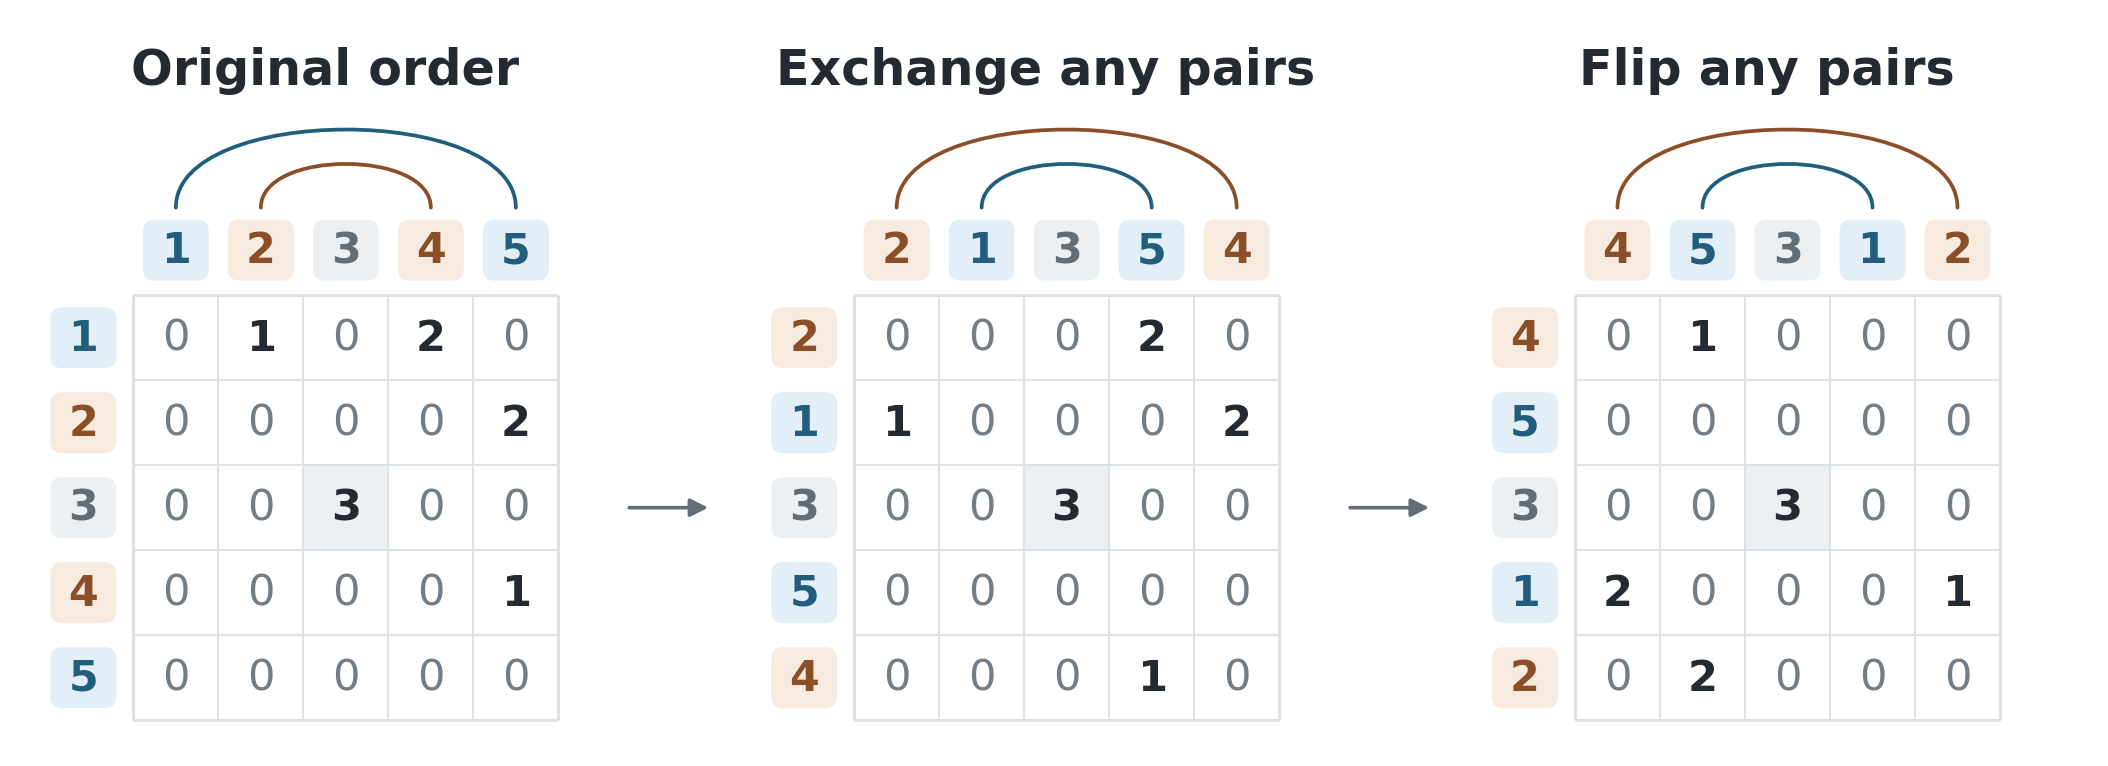
\includegraphics[width=\linewidth]{mirror-pair-rule.png}\par
  \small The arcs track the original pairs $\{1,5\}$ and $\{2,4\}$.
  The middle panel exchanges the pairs. The right panel then flips the
  two indices within each pair. Index $3$ stays in the middle slot.
 \end{minipage}
\end{center}

\newpage
\subsubsection{A four-dimensional worked example}
Use the matrix $P$ from Section~\ref{sec:permutation-matrix}, with ordering $p=(2,1,4,3)$. With
\[
 A=\begin{pmatrix}
 1&2&3&4\\5&6&7&3\\8&9&6&2\\10&8&5&1
 \end{pmatrix},
\]
reordering both rows and columns gives
\[
 P^TAP=\begin{pmatrix}
 6&5&3&7\\2&1&4&3\\8&10&1&5\\9&8&2&6
 \end{pmatrix}.
\]
For example, the new $(1,2)$ and $(3,4)$ entries are both $5$.
The new $(2,1)$ and $(4,3)$ entries are both $2$. All reflected pairs agree.

The ordering $q=(2,1,3,4)$ is invalid because its outer slots contain
$\{2,4\}$, which is absent from $\mathcal C_4$.

\subsubsection{An odd-dimensional example}
The ordering $p=(2,5,3,1,4)$ is valid. The outer slots hold $\{2,4\}$,
the inner pair of slots holds $\{1,5\}$, and slot $3$ holds index $3$.
The ordering $(2,5,1,3,4)$ is invalid because it moves index $3$ and puts
$\{3,5\}$ in the inner pair of slots.

\subsubsection{Connection with graph coupling}
Gupta et al.~\cite[Definition 5.2, p.~29]{gupta-et-al-coupling} call a
partition of an even set of vertices into unordered pairs a \emph{coupling}.
A label is the number assigned to a vertex, which identifies its row
and column in the matrix. With $m$ pairs there are $2m$ labels, and their
relabelings preserve the pairs $\{i,i+m\}$. Reversing the order of the
second half of the labels gives our reversal pairs $\{i,2m+1-i\}$.
For odd $n$, $\mathcal C_n$ is a coupling of the indices other than the middle.

\newpage
\subsection{The complete characterization and proof}
Write $E_{ij}=e_i e_j^T$ for the matrix unit with its $1$ at $(i,j)$.
\begin{theorem}\label{thm:classification}
Let $P$ be an $n\times n$ permutation matrix, with ordering $p$ as defined
in~\eqref{eq:ordering}. The following statements are equivalent:
\begin{enumerate}
 \renewcommand{\labelenumi}{(\roman{enumi})}
 \item $P^TAP$ is persymmetric for every real persymmetric $A$.
 \item $P^TE_{i,r(i)}P$ is persymmetric for every $i=1,\ldots,n$.
 \item $PJ_n=J_n P$.
 \item $P^TJ_n P=J_n$.
 \item $p(n+1-i)=n+1-p(i)$ for every $i$.
\end{enumerate}
\end{theorem}

\begin{proof}
Write the space of real persymmetric $n\times n$ matrices as
\[
 \mathcal S_n=\{A\in\mathbb{R}^{n\times n}:A=J_n A^TJ_n\}.
\]
Reflection across the anti-diagonal leaves each position $(i,r(i))$ in
place. Every other position $(i,j)$ has a distinct reflected position
$(r(j),r(i))$. The two types of positions give two families of matrices.
\begin{itemize}
 \item $\mathcal D_n=\{E_{i,r(i)}:1\leq i\leq n\}$.
   Each has a single $1$ on the anti-diagonal.
 \item $\mathcal R_n=\{E_{ij}+E_{r(j),r(i)}:i+j<n+1\}$.
   Each has a $1$ in two reflected positions. The inequality selects
   the position above the anti-diagonal, so each pair appears once.
\end{itemize}
For example, in size $4$, $E_{14}$ is in $\mathcal D_4$ and
$E_{12}+E_{34}$ is in $\mathcal R_4$. The first uses one position on
the anti-diagonal. The second uses the two positions $(1,2)$ and $(3,4)$,
which reflect to each other.

To build any $A\in\mathcal S_n$, scale each single-entry matrix by the
corresponding entry of $A$ and each two-entry matrix by the value
shared by its reflected entries. Adding the results gives $A$.
This is why $\mathcal D_n\cup\mathcal R_n$ spans $\mathcal S_n$.
For fixed $P$, the map $A\mapsto P^TAP$ is linear, so it is enough to
test these matrices. In fact, the tests on $\mathcal D_n$ will suffice.

\textbf{(i) $\Rightarrow$ (ii).}
If the reordering preserves every persymmetric matrix, it preserves
each $E_{i,r(i)}$. Its single $1$ lies on the anti-diagonal, so it is
persymmetric to begin with.

\newpage
\textbf{(ii) $\Rightarrow$ (iii).}
Assume every $P^TE_{i,r(i)}P$ is persymmetric. For any $i$, this means
\[
 J_n(P^TE_{i,r(i)}P)^TJ_n=P^TE_{i,r(i)}P.
\]
Use $E_{i,r(i)}=e_i e_{r(i)}^T$ and $E_{i,r(i)}^T=e_{r(i)}e_i^T$.
Transposing the product and substituting gives
\[
 J_n P^T e_{r(i)} e_i^T PJ_n=P^T e_i e_{r(i)}^T P.
\]
Grouping each side into a column times a row gives
\[
 \underbrace{(J_n P^T e_{r(i)})}_{\text{column}}\,
 \underbrace{(e_i^T PJ_n)}_{\text{row}}
 =
 \underbrace{(P^T e_i)}_{\text{column}}\,
 \underbrace{(e_{r(i)}^T P)}_{\text{row}}.
\]
Each factor is a vector with a single $1$ because multiplying by a
permutation matrix just moves the $1$ in the original basis vector.
The product has a single $1$ at the row picked by the column factor
and the column picked by the row factor. Since the products are equal,
the $1$ is in the same row on both sides. The column factors therefore satisfy
\[
 J_n P^T e_{r(i)}=P^T e_i.
\]

Since $e_{r(i)}=J_n e_i$, this is $(J_n P^TJ_n)e_i=P^Te_i$ for every $i$.
Multiplying a matrix by $e_i$ selects its $i$th column. Since the
equality holds for every $i$, it gives the first line below.
\begin{align*}
 J_n P^TJ_n &= P^T && \text{(compare all columns)},\\
 J_n PJ_n &= P && \text{(transpose and use $J_n^T=J_n$)},\\
 J_n P &= PJ_n && \text{(multiply on the right by $J_n$ and use $J_n^2=I_n$)}.
\end{align*}

\textbf{(iii) $\Rightarrow$ (i).}
Assume $PJ_n=J_n P$ and take any $A\in\mathcal S_n$.
Transposing $PJ_n=J_n P$ shows that $P^T$ also commutes with $J_n$.
We can therefore move each $J_n$ next to $A^T$ in the calculation.
\begin{align*}
 J_n(P^TAP)^TJ_n
 &=J_n P^T A^T PJ_n\\
 &=P^T(J_n A^TJ_n)P\\
 &=P^TAP.
\end{align*}
The last step uses $J_n A^TJ_n=A$. Thus $P^TAP$ is persymmetric.

\textbf{(iii) $\Leftrightarrow$ (iv).}
Multiply $PJ_n=J_n P$ on the left by $P^T$ to obtain
$P^TPJ_n=P^TJ_n P$. Since $P^TP=I_n$, this is $J_n=P^TJ_n P$.
In the other direction, multiply on the left by $P$ and use
$PP^T=I_n$ to recover $PJ_n=J_n P$.

\textbf{(iii) $\Leftrightarrow$ (v).}
Apply both products to $e_i$. Using $Pe_i=e_{p(i)}$ and $J_n e_i=e_{r(i)}$
gives
\[
 PJ_n e_i=P e_{r(i)}=e_{p(r(i))},
 \qquad
 J_n P e_i=J_n e_{p(i)}=e_{r(p(i))}.
\]
The products agree column by column exactly when the two indices agree
for every $i$. Substituting $r(i)=n+1-i$ into $p(r(i))=r(p(i))$
gives $p(n+1-i)=n+1-p(i)$, the mirror rule.

The first three implications form a loop, and the last two link (iv)
and (v) to (iii). Thus all five conditions are equivalent.
\[
 \text{(i)}\Rightarrow\text{(ii)}\Rightarrow\text{(iii)}\Rightarrow\text{(i)},
 \qquad
 \text{(iii)}\Leftrightarrow\text{(iv)},
 \qquad
 \text{(iii)}\Leftrightarrow\text{(v)}.\qedhere
\]
\end{proof}

\newpage
\subsection{How many permutations are there?}
Let $m=\lfloor n/2\rfloor$. There are $m$ mirror pairs. Choose an ordering
of those pairs in $m!$ ways, then choose the orientation of each pair in
$2^m$ ways. When $n$ is odd, the middle index has no choice: it stays fixed.
Consequently,
\[
 \boxed{\#\{P:\ P^TAP\text{ preserves persymmetry for every }A\}
 =2^{\lfloor n/2\rfloor}\lfloor n/2\rfloor!.}
\]
\begin{center}
\begin{tabular}{rrr}
\toprule
Dimension $n$ & All permutations $n!$ & Permitted permutations\\
\midrule
1&1&1\\2&2&2\\3&6&2\\4&24&8\\5&120&8\\6&720&48\\7&5040&48\\
\bottomrule
\end{tabular}
\end{center}
In dimension $2$, both permutations work. In dimension $3$, the middle
index must stay fixed, and the only possibilities are $I_3$ and $J_3$.

\subsubsection{All eight orderings in dimension 4}
Under our convention, the permitted lists are
\[
\begin{array}{llll}
(1,2,3,4),&(1,3,2,4),&(2,1,4,3),&(2,4,1,3),\\[2pt]
(3,1,4,2),&(3,4,1,2),&(4,2,3,1),&(4,3,2,1).
\end{array}
\]
Notice that not every valid permutation is its own inverse.
For $p=(2,4,1,3)$,
\[
 P=\begin{pmatrix}0&0&1&0\\1&0&0&0\\0&0&0&1\\0&1&0&0\end{pmatrix},
\]
which commutes with $J_4$ but satisfies $P^T\ne P$. Thus replacing $P^T$
by $P$ in a calculation is not justified in general.


\newpage
\subsection{Consequences for eigenvalues and nilpotency}
Since $P^{-1}=P^T$, the matrices $A$ and $B=P^TAP$ are similar. For example,
\begin{align*}
 \det(xI-B)
 &=\det\bigl(P^T(xI-A)P\bigr)\\
 &=\det(P^T)\det(xI-A)\det(P)\\
 &=\det(xI-A).
\end{align*}
They therefore have the same characteristic polynomial and eigenvalues,
including multiplicities. Also,
\[
 B^2=P^TAP\,P^TAP=P^TA^2P,
 \qquad B^k=P^TA^kP.
\]
Thus $A^k=0$ if and only if $B^k=0$. For instance,
\[
 U=\begin{pmatrix}0&1&0\\0&0&1\\0&0&0\end{pmatrix},
 \qquad J_3^TUJ_3=
 \begin{pmatrix}0&0&0\\1&0&0\\0&1&0\end{pmatrix}.
\]
Both matrices are persymmetric, have characteristic polynomial $x^3$, and
have cube zero but square nonzero. The upper-shift and lower-shift patterns
represent the same case under an admissible permutation.

\bibliographystyle{plain}
\begingroup
\raggedright
\bibliography{references}
\endgroup

\end{document}
